\documentclass{extbook}[14pt]
\usepackage{multicol, enumerate, enumitem, hyperref, color, soul, setspace, parskip, fancyhdr, amssymb, amsthm, amsmath, bbm, latexsym, units, mathtools}
\everymath{\displaystyle}
\usepackage[headsep=0.5cm,headheight=0cm, left=1 in,right= 1 in,top= 1 in,bottom= 1 in]{geometry}
\usepackage{dashrule}  % Package to use the command below to create lines between items
\newcommand{\litem}[1]{\item #1

\rule{\textwidth}{0.4pt}}
\pagestyle{fancy}
\lhead{}
\chead{Answer Key for Progress Quiz 4 Version C}
\rhead{}
\lfoot{8448-1521}
\cfoot{}
\rfoot{Fall 2020}
\begin{document}
\textbf{This key should allow you to understand why you choose the option you did (beyond just getting a question right or wrong). \href{https://xronos.clas.ufl.edu/mac1105spring2020/courseDescriptionAndMisc/Exams/LearningFromResults}{More instructions on how to use this key can be found here}.}

\textbf{If you have a suggestion to make the keys better, \href{https://forms.gle/CZkbZmPbC9XALEE88}{please fill out the short survey here}.}

\textit{Note: This key is auto-generated and may contain issues and/or errors. The keys are reviewed after each exam to ensure grading is done accurately. If there are issues (like duplicate options), they are noted in the offline gradebook. The keys are a work-in-progress to give students as many resources to improve as possible.}

\rule{\textwidth}{0.4pt}

\begin{enumerate}\litem{
Construct the lowest-degree polynomial given the zeros below. Then, choose the intervals that contain the coefficients of the polynomial in the form $ax^3+bx^2+cx+d$.
\[ \frac{3}{2}, -6, \text{ and } \frac{5}{3} \]
The solution is \( 6x^{3} +17 x^{2} -99 x + 90 \), which is option E.\begin{enumerate}[label=\Alph*.]
\item \( a \in [5, 11], b \in [34, 42], c \in [-24, -15], \text{ and } d \in [-99, -85] \)

$6x^{3} +35 x^{2} -21 x -90$, which corresponds to multiplying out $(2x + 2)(x -1)(3x -3)$.
\item \( a \in [5, 11], b \in [14, 18], c \in [-103, -96], \text{ and } d \in [-99, -85] \)

$6x^{3} +17 x^{2} -99 x -90$, which corresponds to multiplying everything correctly except the constant term.
\item \( a \in [5, 11], b \in [-22, -16], c \in [-103, -96], \text{ and } d \in [-99, -85] \)

$6x^{3} -17 x^{2} -99 x -90$, which corresponds to multiplying out $(2x + 3)(x -6)(3x + 5)$.
\item \( a \in [5, 11], b \in [-41, -32], c \in [-11, -3], \text{ and } d \in [87, 95] \)

$6x^{3} -37 x^{2} -9 x + 90$, which corresponds to multiplying out $(2x + 2)(x + 1)(3x -3)$.
\item \( a \in [5, 11], b \in [14, 18], c \in [-103, -96], \text{ and } d \in [87, 95] \)

* $6x^{3} +17 x^{2} -99 x + 90$, which is the correct option.
\end{enumerate}

\textbf{General Comment:} To construct the lowest-degree polynomial, you want to multiply out $(2x -3)(x + 6)(3x -5)$
}
\litem{
Describe the zero behavior of the zero $x = 3$ of the polynomial below.
\[ f(x) = 6(x - 6)^{10}(x + 6)^{9}(x + 3)^{12}(x - 3)^{7} \]
The solution is the graph below, which is option D.
\begin{center}
    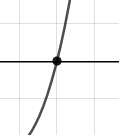
\includegraphics[width=0.3\textwidth]{../Figures/polyZeroBehaviorCopyDC.png}
\end{center}\begin{enumerate}[label=\Alph*.]
\begin{multicols}{2}
\item 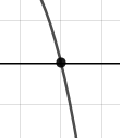
\includegraphics[width = 0.3\textwidth]{../Figures/polyZeroBehaviorCopyAC.png}
\item 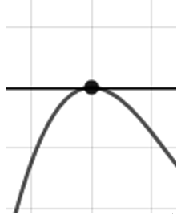
\includegraphics[width = 0.3\textwidth]{../Figures/polyZeroBehaviorCopyBC.png}
\item 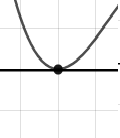
\includegraphics[width = 0.3\textwidth]{../Figures/polyZeroBehaviorCopyCC.png}
\item 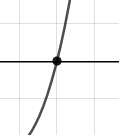
\includegraphics[width = 0.3\textwidth]{../Figures/polyZeroBehaviorCopyDC.png}
\end{multicols}\item None of the above.\end{enumerate}
\textbf{General Comment:} You will need to sketch the entire graph, then zoom in on the zero the question asks about.
}
\litem{
Construct the lowest-degree polynomial given the zeros below. Then, choose the intervals that contain the coefficients of the polynomial in the form $ax^3+bx^2+cx+d$.
\[ 6, 4, \text{ and } \frac{5}{4} \]
The solution is \( 4x^{3} -45 x^{2} +146 x -120 \), which is option A.\begin{enumerate}[label=\Alph*.]
\item \( a \in [4, 8], b \in [-48, -38], c \in [139, 147], \text{ and } d \in [-122, -114] \)

* $4x^{3} -45 x^{2} +146 x -120$, which is the correct option.
\item \( a \in [4, 8], b \in [-1, 4], c \in [-110, -99], \text{ and } d \in [117, 124] \)

$4x^{3} +3 x^{2} -106 x + 120$, which corresponds to multiplying out $(x + 1)(x -1)(4x -4)$.
\item \( a \in [4, 8], b \in [-48, -38], c \in [139, 147], \text{ and } d \in [117, 124] \)

$4x^{3} -45 x^{2} +146 x + 120$, which corresponds to multiplying everything correctly except the constant term.
\item \( a \in [4, 8], b \in [45, 46], c \in [139, 147], \text{ and } d \in [117, 124] \)

$4x^{3} +45 x^{2} +146 x + 120$, which corresponds to multiplying out $(x + 6)(x + 4)(4x + 5)$.
\item \( a \in [4, 8], b \in [29, 37], c \in [42, 52], \text{ and } d \in [-122, -114] \)

$4x^{3} +35 x^{2} +46 x -120$, which corresponds to multiplying out $(x + 1)(x + 1)(4x -4)$.
\end{enumerate}

\textbf{General Comment:} To construct the lowest-degree polynomial, you want to multiply out $(x -6)(x -4)(4x -5)$
}
\litem{
Construct the lowest-degree polynomial given the zeros below. Then, choose the intervals that contain the coefficients of the polynomial in the form $x^3+bx^2+cx+d$.
\[ -4 + 4 i \text{ and } 2 \]
The solution is \( x^{3} +6 x^{2} +16 x -64 \), which is option D.\begin{enumerate}[label=\Alph*.]
\item \( b \in [0, 1.3], c \in [-8, -4], \text{ and } d \in [1, 15] \)

$x^{3} + x^{2} -6 x + 8$, which corresponds to multiplying out $(x -4)(x -2)$.
\item \( b \in [0, 1.3], c \in [0, 4], \text{ and } d \in [-15, -3] \)

$x^{3} + x^{2} +2 x -8$, which corresponds to multiplying out $(x + 4)(x -2)$.
\item \( b \in [-7.3, -2], c \in [12, 25], \text{ and } d \in [64, 74] \)

$x^{3} -6 x^{2} +16 x + 64$, which corresponds to multiplying out $(x-(-4 + 4 i))(x-(-4 - 4 i))(x + 2)$.
\item \( b \in [4.2, 7.3], c \in [12, 25], \text{ and } d \in [-64, -61] \)

* $x^{3} +6 x^{2} +16 x -64$, which is the correct option.
\item \( \text{None of the above.} \)

This corresponds to making an unanticipated error or not understanding how to use nonreal complex numbers to create the lowest-degree polynomial. If you chose this and are not sure what you did wrong, please contact the coordinator for help.
\end{enumerate}

\textbf{General Comment:} Remember that the conjugate of $a+bi$ is $a-bi$. Since these zeros always come in pairs, we need to multiply out $(x-(-4 + 4 i))(x-(-4 - 4 i))(x-(2))$.
}
\litem{
Construct the lowest-degree polynomial given the zeros below. Then, choose the intervals that contain the coefficients of the polynomial in the form $x^3+bx^2+cx+d$.
\[ -2 - 5 i \text{ and } 4 \]
The solution is \( x^{3} +13 x -116 \), which is option C.\begin{enumerate}[label=\Alph*.]
\item \( b \in [-1.34, 0.32], c \in [12.8, 14.7], \text{ and } d \in [113, 118] \)

$x^{3} +13 x + 116$, which corresponds to multiplying out $(x-(-2 - 5 i))(x-(-2 + 5 i))(x + 4)$.
\item \( b \in [0.71, 1.99], c \in [-2.2, -0.1], \text{ and } d \in [-13, -3] \)

$x^{3} + x^{2} -2 x -8$, which corresponds to multiplying out $(x + 2)(x -4)$.
\item \( b \in [-1.34, 0.32], c \in [12.8, 14.7], \text{ and } d \in [-121, -114] \)

* $x^{3} +13 x -116$, which is the correct option.
\item \( b \in [0.71, 1.99], c \in [-1.7, 1.2], \text{ and } d \in [-24, -19] \)

$x^{3} + x^{2} +x -20$, which corresponds to multiplying out $(x + 5)(x -4)$.
\item \( \text{None of the above.} \)

This corresponds to making an unanticipated error or not understanding how to use nonreal complex numbers to create the lowest-degree polynomial. If you chose this and are not sure what you did wrong, please contact the coordinator for help.
\end{enumerate}

\textbf{General Comment:} Remember that the conjugate of $a+bi$ is $a-bi$. Since these zeros always come in pairs, we need to multiply out $(x-(-2 - 5 i))(x-(-2 + 5 i))(x-(4))$.
}
\litem{
Which of the following equations \textit{could} be of the graph presented below?

\begin{center}
    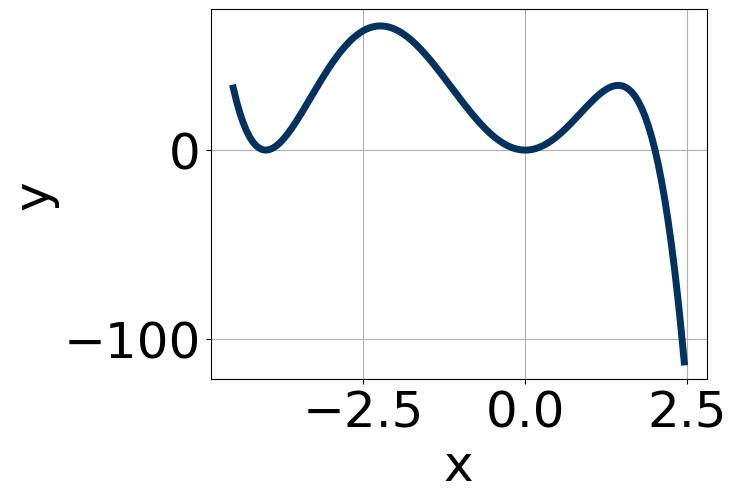
\includegraphics[width=0.5\textwidth]{../Figures/polyGraphToFunctionCopyC.png}
\end{center}



The solution is \( -17x^{10} (x + 4)^{8} (x - 2)^{9} \), which is option B.\begin{enumerate}[label=\Alph*.]
\item \( 9x^{6} (x + 4)^{4} (x - 2)^{5} \)

This corresponds to the leading coefficient being the opposite value than it should be.
\item \( -17x^{10} (x + 4)^{8} (x - 2)^{9} \)

* This is the correct option.
\item \( -9x^{10} (x + 4)^{7} (x - 2)^{4} \)

The factor $(x + 4)$ should have an even power and the factor $(x - 2)$ should have an odd power.
\item \( 5x^{10} (x + 4)^{8} (x - 2)^{6} \)

The factor $(x - 2)$ should have an odd power and the leading coefficient should be the opposite sign.
\item \( -10x^{10} (x + 4)^{7} (x - 2)^{9} \)

The factor $(x + 4)$ should have an even power.
\end{enumerate}

\textbf{General Comment:} General Comments: Draw the x-axis to determine which zeros are touching (and so have even multiplicity) or cross (and have odd multiplicity).
}
\litem{
Which of the following equations \textit{could} be of the graph presented below?

\begin{center}
    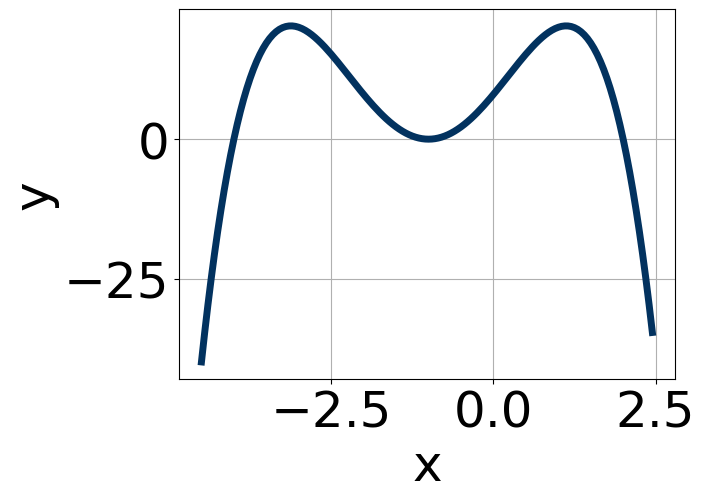
\includegraphics[width=0.5\textwidth]{../Figures/polyGraphToFunctionC.png}
\end{center}



The solution is \( -16(x + 1)^{4} (x + 4)^{9} (x - 2)^{9} \), which is option E.\begin{enumerate}[label=\Alph*.]
\item \( -10(x + 1)^{9} (x + 4)^{8} (x - 2)^{9} \)

The factor $-1$ should have an even power and the factor $-4$ should have an odd power.
\item \( -16(x + 1)^{6} (x + 4)^{6} (x - 2)^{5} \)

The factor $(x + 4)$ should have an odd power.
\item \( 12(x + 1)^{4} (x + 4)^{9} (x - 2)^{7} \)

This corresponds to the leading coefficient being the opposite value than it should be.
\item \( 5(x + 1)^{8} (x + 4)^{5} (x - 2)^{10} \)

The factor $(x - 2)$ should have an odd power and the leading coefficient should be the opposite sign.
\item \( -16(x + 1)^{4} (x + 4)^{9} (x - 2)^{9} \)

* This is the correct option.
\end{enumerate}

\textbf{General Comment:} General Comments: Draw the x-axis to determine which zeros are touching (and so have even multiplicity) or cross (and have odd multiplicity).
}
\litem{
Describe the end behavior of the polynomial below.
\[ f(x) = -4(x - 4)^{2}(x + 4)^{7}(x - 7)^{3}(x + 7)^{4} \]
The solution is the graph below, which is option B.
\begin{center}
    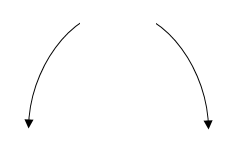
\includegraphics[width=0.3\textwidth]{../Figures/polyEndBehaviorBC.png}
\end{center}\begin{enumerate}[label=\Alph*.]
\begin{multicols}{2}
\item 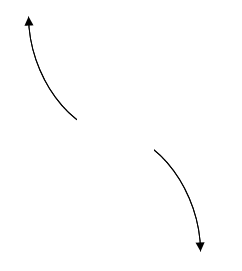
\includegraphics[width = 0.3\textwidth]{../Figures/polyEndBehaviorAC.png}
\item 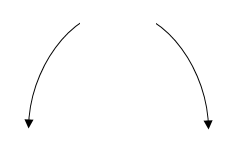
\includegraphics[width = 0.3\textwidth]{../Figures/polyEndBehaviorBC.png}
\item 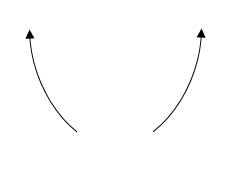
\includegraphics[width = 0.3\textwidth]{../Figures/polyEndBehaviorCC.png}
\item 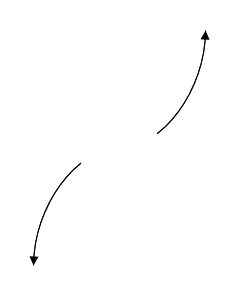
\includegraphics[width = 0.3\textwidth]{../Figures/polyEndBehaviorDC.png}
\end{multicols}\item None of the above.\end{enumerate}
\textbf{General Comment:} Remember that end behavior is determined by the leading coefficient AND whether the \textbf{sum} of the multiplicities is positive or negative.
}
\litem{
Describe the zero behavior of the zero $x = -3$ of the polynomial below.
\[ f(x) = 7(x - 3)^{9}(x + 3)^{10}(x + 4)^{9}(x - 4)^{13} \]
The solution is the graph below, which is option C.
\begin{center}
    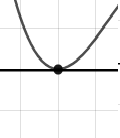
\includegraphics[width=0.3\textwidth]{../Figures/polyZeroBehaviorCC.png}
\end{center}\begin{enumerate}[label=\Alph*.]
\begin{multicols}{2}
\item 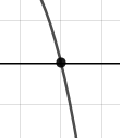
\includegraphics[width = 0.3\textwidth]{../Figures/polyZeroBehaviorAC.png}
\item 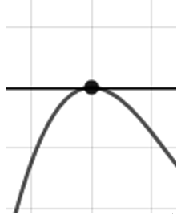
\includegraphics[width = 0.3\textwidth]{../Figures/polyZeroBehaviorBC.png}
\item 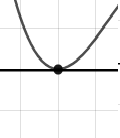
\includegraphics[width = 0.3\textwidth]{../Figures/polyZeroBehaviorCC.png}
\item 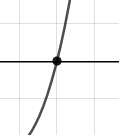
\includegraphics[width = 0.3\textwidth]{../Figures/polyZeroBehaviorDC.png}
\end{multicols}\item None of the above.\end{enumerate}
\textbf{General Comment:} You will need to sketch the entire graph, then zoom in on the zero the question asks about.
}
\litem{
Describe the end behavior of the polynomial below.
\[ f(x) = 2(x + 4)^{2}(x - 4)^{5}(x + 2)^{3}(x - 2)^{5} \]
The solution is the graph below, which is option D.
\begin{center}
    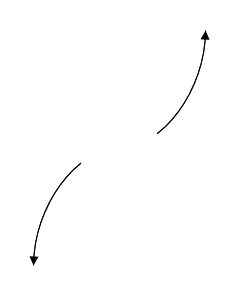
\includegraphics[width=0.3\textwidth]{../Figures/polyEndBehaviorCopyDC.png}
\end{center}\begin{enumerate}[label=\Alph*.]
\begin{multicols}{2}
\item 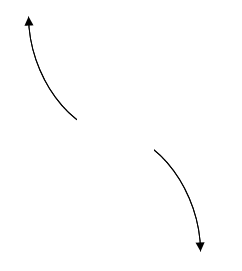
\includegraphics[width = 0.3\textwidth]{../Figures/polyEndBehaviorCopyAC.png}
\item 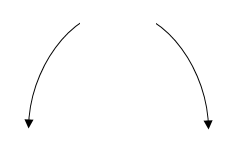
\includegraphics[width = 0.3\textwidth]{../Figures/polyEndBehaviorCopyBC.png}
\item 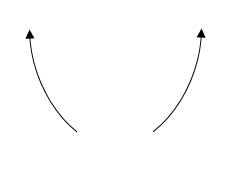
\includegraphics[width = 0.3\textwidth]{../Figures/polyEndBehaviorCopyCC.png}
\item 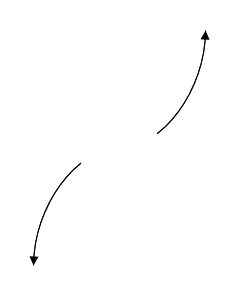
\includegraphics[width = 0.3\textwidth]{../Figures/polyEndBehaviorCopyDC.png}
\end{multicols}\item None of the above.\end{enumerate}
\textbf{General Comment:} Remember that end behavior is determined by the leading coefficient AND whether the \textbf{sum} of the multiplicities is positive or negative.
}
\end{enumerate}

\end{document}